\documentclass[12pt]{article}

\usepackage{enumitem}
\usepackage[right=20mm, left=20mm]{geometry}
\usepackage{type1cm}
\usepackage{amssymb}
\usepackage[fleqn]{amsmath}
\usepackage{tikz}
\usepackage{multicol}
\usepackage{makecell}
\setlength{\columnsep}{1pt}
\usepackage{pgfplots}
\usepackage{float}
\usepackage{caption}
\usepackage{subcaption}
% \usepackage{subfig}
\usepackage{graphicx}
\usepackage{array}

\usepackage{indentfirst}
\usepackage{lastpage}  
\usepackage{fancyhdr}
\pagestyle{fancy}

\usepackage[unicode=true,pdfusetitle,
 bookmarks=true,bookmarksnumbered=false,bookmarksopen=false,
 breaklinks=false,pdfborder={0 0 1},backref=false,colorlinks=false]
 {hyperref}

\makeatletter
\newenvironment{myalign*}{\ifvmode\else\hfil\null\linebreak\fi
  \hspace*{-\leftmargin}\minipage\textwidth
  \setlength{\abovedisplayskip}{0pt}%
  \setlength{\abovedisplayshortskip}{\abovedisplayskip}%
  \start@align\@ne\st@rredtrue\m@ne}%
{\endalign\endminipage\linebreak}

% Paper size
\topmargin -10mm
\textwidth 170mm
% \oddsidemargin -5mm
% \evensidemargin -5mm
\textheight 220mm

% Font setting
\usepackage{xeCJK}
% \setCJKmainfont{Noto Sans TC}
\setCJKmainfont{kaiu.ttf}


\renewcommand{\footnotesize}{\normalsize} 
\renewcommand{\headrulewidth}{0pt}
\renewcommand{\footrulewidth}{0pt}

\lhead{}
\chead{2023年全國大專校院智慧創新暨跨域整合創作競賽系統需求書}
\rhead{}

\lfoot{}
\cfoot{}
\rfoot{ 共 \pageref{LastPage} 頁 第  \thepage   頁} 

\makeatletter
\begin{document}
% \fontsize{14pt}{18pt}\selectfont
% \author{}
\date{}
\usetikzlibrary{automata, positioning, arrows}
% \maketitle
\tikzset{every state, accepting/.style={double distance=2pt}}
\captionsetup[figure]{labelfont={bf},name={圖},labelsep=period}
\renewcommand{\arraystretch}{1.45}

\noindent
\textbf{參賽隊名:} 普羅程式 \\
\textbf{作品名稱:} 威力導師 PowerTeacher \\
\textbf{系統名稱:} 威力導師

\section{系統目的與範圍}

PowerTeacher 的主要目的在於成為一個永續發展的教育解決方案,推動聯合國的17項永續發展目標,特別專注於「SDG 4 優質教育」和「SDG 9 產業、創新與基礎設施」。這個系統旨在解決台灣基層教育中程式教學所面臨的問題,例如傳統教學方式的不足、學生狀況即時追蹤困難以及軟硬體設施使用困難等。PowerTeacher 的範圍涵蓋國高中的基礎程式教學,提供一個全面的教學模組,整合了直播、實作、測驗、互動等元素,並支援多達60種不同的程式語言,以滿足多樣化的教學需求。同時,系統融合了影音剪輯軟體的腳本式設計邏輯,讓講義編輯變得直覺且視覺化,使所有使用者都能輕鬆地進行優質的程式教學。該系統以網頁應用形式呈現,提供三種主要頁面,用以支援教師進行不同的教學活動。\\

\begin{figure}[H]
  \centering
  \begin{subfigure}{0.4\linewidth}
    \centering
    \href{https://raw.githubusercontent.com/programingtw/proglearn-plan/main/2023全國大專校院智慧創新暨跨域整合創作競賽/img/E_SDG_PRINT-04.jpg}{ 
      
\includegraphics[width=1\textwidth]{./img/E_SDG_PRINT-04.jpg}
    }
    \caption{SDG 4 優質教育:確保包容和公平的優質教育,讓全民享有終身學習的機會}
  \end{subfigure}
  \label{arc1}
  \begin{subfigure}{0.4\linewidth}
    \centering
    \href{https://raw.githubusercontent.com/programingtw/proglearn-plan/main/2023全國大專校院智慧創新暨跨域整合創作競賽/img/E_SDG_PRINT-09.jpg}{ 
      
\includegraphics[width=1\textwidth]{./img/E_SDG_PRINT-09.jpg}
    }
    \caption{SDG 9 產業、創新與基礎設施:建設具有韌性的基礎設施,促進包容性和永續的工業化}
  \end{subfigure}
  \label{arc2}
  \caption{聯合國永續發展目標 SDGs 目標 (點擊可看大圖)。圖片來源:\href{https://www.un.org/sustainabledevelopment/news/communications-material/}{聯合國}}
\end{figure}

\section{系統非功能需求}
\begin{table}[H]
  \centering
  \begin{tabular}{|c|p{15cm}|}
    \hline
    \textbf{代號} & \textbf{非功能需求} \\
    \hline
    NFR-001 & 使用者介面與人為因素 \\ 
    & $\bullet$ 使用者:程式設計課程的老師、學生 \\
    & $\bullet$ 使用者的介面設計:簡單並且易上手、高度的功能整合、即時獲得使用者的反饋與資訊。 \\
    & $\bullet$ 使用者的引導與教學:直觀的 UI 設計並且將編輯功能視覺化。\\
    \hline
    NFR-002 & 設備需求 \\
    & $\bullet$ 使用者的使用設備:使用設備以電腦為主、手持設備為輔,並針對電腦使用最佳化。\\
    & $\bullet$ 使用者的設備限制:所有能瀏覽網頁的設備皆可使用。\\
    \hline
    NFR-003 & 效能需求 \\
    & $\bullet$ 反應時間:同一課程能讓 100 人同時使用,並在 0.1 秒內回應使用者。\\
    & $\bullet$ 容量限制:限制每位教師在單一章節中,只能上傳 20MB 以下的投影片。\\
    & $\bullet$ 課堂限制:每位教師的課程需要經過管理員審核後才能開課,並且每位教師以開設 5 門課為限。\\
    & $\bullet$ 課堂人數:同一課程最多只能有 100 位學生。\\
    \hline
    NFR-004 & 錯誤處理 \\
    & $\bullet$ 系統遇到不正常的負載:針對大量請求的用戶限制封包的流量。\\
    & $\bullet$ 系統遇到高負載:使用排隊來限制同時登入人數。\\
    \hline
    % 在這裡添加其他非功能需求...
    % NFR-002, NFR-003, ...
    % 將其他需求按相同的格式添加到表格中
  \end{tabular}
\end{table}

\section{系統功能需求}

\begin{table}[H]
  \centering
  \begin{tabular}{|c|p{15cm}|}
    \hline
    \textbf{代號} & \textbf{功能需求} \\
    \hline
    FR-001 & 會員系統 - 使用已註冊的帳號密碼登入系統,可以查看所有課程及其詳細資訊 \\  \hline
    FR-002 & 使用者個人資料設定 - 使用者可以設定及修改個人資料和密碼 \\  \hline
    FR-003 & 所有課程 - 提供使用者查看目前所有的課程 \\  \hline
    FR-004 & 新增課程 - 教師可以新增課程並填寫課程基本內容 \\  \hline
    FR-005 & 編輯課程 - 教師可以編輯課程資訊並管理學生 \\  \hline
    FR-006 & 所有章節 - 使用者可以查看課程內每個章節的講義、教材和詳細資訊,章節以階層結構顯示 \\  \hline
    FR-007 & 新增章節 - 教師可以新增章節,填寫章節內容並上傳投影片 \\  \hline
    FR-008 & 新增作業 - 教師可以新增作業,使用練習區的練習題或自己寫題目 \\  \hline
    FR-009 & 新增公告 - 教師可以新增公告,設定發送對象 \\  \hline
    FR-010 & 上傳教材 - 教師可以上傳教材,選擇上傳檔案類型 \\  \hline
    FR-011 & 下載教材 - 學生可以點擊教材進行下載 \\  \hline
    FR-012 & 互動式講義 - 使用者可以查看該章節講義的補充說明,練習題目,跟隨老師的上課進度 \\  \hline
    FR-013 & 編輯互動講義 - 教師可以編輯互動講義,以積木方式分塊內容,並以時間軸編輯方法控制顯示區段 \\  \hline
    FR-014 & 引導模式 - 學生在引導模式下,可以看到以黃色區塊標示的老師當前進度 \\  \hline
    FR-015 & 練習題目 - 學生可以進行題目練習並提交查看結果 \\  \hline
    FR-016 & 教學頁面 - 使用者可以查看該堂課程的直播以及記錄檔 \\  \hline
    FR-017 & 觀看直播、章節概述以及互動式講義 - 學生可以查看直播、章節概述以及互動式講義 \\  \hline
    FR-018 & 查看講義以及學生作答狀況 - 老師可以查看講義以及學生對於練習題的作答狀況 \\  \hline
    FR-019 & 開啟同步 - 老師可以開啟同步功能,紀錄上課資訊 \\  \hline
    FR-020 & 練習題 - 老師與學生可以查看課後作業的練習題列表,並進入單個題目的詳細頁面。\\ \hline
    FR-021 & 查看題目作答結果 - 學生可以查看自己的題目作答結果。 \\ \hline
    FR-022 & 查看所有學生的作答結果 - 老師可以查看所有學生繳交的該題目的作答結果。 \\ \hline 
    FR-023 & 查看作答結果統計 - 老師可以查看所有學生的作答結果統計。 \\ \hline
  \end{tabular}
\end{table}

\section{Use Case Model}

\begin{table}[H]
  \centering
  \begin{tabular}{|l|p{14cm}|}
  \hline
  \textbf{使用案例名稱} & 老師編輯講義 \\ 
  \hline
  \textbf{參與者} & 老師(王大明)、威力導師系統 \\ 
  \hline
  \textbf{前置條件} & 王大明打算編輯下一節課的講義。他已經為該課程創建了章節並上傳了講義。\\ 
  \hline
  \textbf{事件流程} 
  & 1. 王大明進入網頁,由於登入已經過期所以需要重新登入。他在輸入帳號以及密碼之後點擊登入按鈕來進行登入,並進入主畫面。 \\
  & 2. 系統驗證王大明的帳號密碼後,並且回傳課程列表給王大明。 \\
  & 3. 王大明點擊他需要準備的課程卡片,進入該課程的章節列表編輯頁面。 \\
  & 4. 系統回傳並顯示該課程的所有章節列表給王大明。 \\
  & 5. 王大明點擊他要編輯的講義,進入該講義的頁面。 \\
  & 6. 在講義頁面,王大明選擇編輯按鈕,進入該講義的編輯頁面。 \\
  & 7. 王大明點擊添加程式碼練習題方塊,使用 markdown 輸入題目敘述,並輸入帶有空格的 C++ 程式碼題目。 \\
  & 8. 王大明為程式碼練習題添加答案選項。 \\
  & 9. 王大明編輯完題目後,按下測試執行按鈕。 \\
  & 10. 系統回傳練習題測試結果給王大明。 \\
  & 11. 王大明確認測試結果無誤後,將程式碼練習題方塊拖曳到時間軸並調整其跨度。 \\ 
  & 12. 他將編輯好的講義儲存,或者在需要處理其他事情時暫時儲存當前的變更。 \\
  \hline
  \textbf{例外處理} 
  & 若在事件流程10中,系統回傳錯誤的測試結果或出現問題,他將無法確認題目的正確性。這時,王大明可以重新編輯題目或請求技術支援。系統應提供錯誤信息以幫助他找到問題所在。 \\
  & 若在事件流程12中,無法儲存變更,此時,系統應該提示錯誤信息,讓他知道出了什麼問題,並嘗試解決它。 \\
  \hline
  \textbf{後置條件} & 王大明完成講義的編輯,並且成功保存了他的變更。學生可以看到更新後的講義並進行學習。 \\
  \hline
  \end{tabular}
\end{table}

\begin{table}[H]
  \centering
  \begin{tabular}{|l|p{14cm}|}
  \hline
  \textbf{使用案例名稱} & 老師上課 \\ 
  \hline
  \textbf{參與者} & 老師(王大明)、威力導師系統 \\ 
  \hline
  \textbf{前置條件} & 王大明已登入威力導師系統並已經完成課程的準備,準備開始上課。 \\ 
  \hline
  \textbf{事件流程} 
  & 1. 系統顯示主畫面,給王大明展示所有課程的卡片及新增課程的卡片。 \\
  & 2. 王大明選擇並點擊即將開課的課程卡片,系統將他導向該課程的教學頁面。 \\
  & 3. 系統回傳投影片、互動式講義、章節概述、練習題目等資訊給王大明。 \\
  & 4. 在教學頁面,王大明點擊"開始授課"按鈕,並開始進行授課。 \\
  & 5. 系統將課程狀態改為同步模式,並開始記錄所有活動。 \\
  & 6. 授課過程中,當每個段落結束時,王大明給予學生練習題目。 \\
  & 7. 學生作答完成後,系統將回傳學生的答題情況,王大明會依據結果針對性講解練習題。 \\
  & 6. 授課結束後,王大明點擊"結束授課"按鈕,將課程狀態設定為非同步模式。 \\ 
  \hline
  \textbf{例外處理} 
  & 若在事件流程2中,王大明點擊了不存在的課程卡片,系統將會回到主頁面並給他顯示錯誤訊息。 \\
  & 若在事件流程4中,由於網路問題,王大明無法將課程狀態設定為同步模式,此時,系統將提示他檢查網路連線情況。 \\
  & 若在事件流程7中,由於網路問題,王大明無法獲得學生的答題情況,此時,系統將提示他檢查網路連線情況。 \\
  \hline
  \textbf{後置條件} 
  & 王大明成功完成一次授課,課程狀態已改為非同步。系統記錄並儲存此次授課的所有活動和學生的學習狀況。 \\
  \hline
  \end{tabular}
\end{table}

\begin{table}[H]
  \centering
  \begin{tabular}{|l|p{14cm}|}
  \hline
  \textbf{使用案例名稱} & 學生上課 \\ 
  \hline
  \textbf{參與者} & 學生(王小明)、威力導師系統 \\ 
  \hline
  \textbf{前置條件} & 王小明已登入威力導師系統並準備參加即將開始的課程。 \\ 
  \hline
  \textbf{事件流程} 
  & 1. 王小明開啟威力導師系統的網頁,由於他已經登入,系統自動導向主畫面。 \\
  & 2. 系統會回傳並顯示所有課程的卡片給王小明。 \\
  & 3. 王小明點選正在進行中的課程卡片,並直接進入該課程的教學頁面。 \\
  & 4. 系統回傳投影片、互動式講義、章節概述、練習題目等資訊給王小明。 \\
  & 5. 王小明發現目前老師講解的內容他已經理解,由於老師開放了預習,他決定點選投影片的其他部分進行預習。 \\
  & 6. 王小明預習完後決定回到老師目前講解的進度,他點擊"回到當前進度"按鈕,跟隨老師的進度學習,同時互動式講義也會引導到與老師的相同進度。 \\
  & 7. 老師在一個段落結束後,給予了一個程式碼練習題供學生練習。王小明仔細讀過題目,選擇他認為正確的答案並點擊"提交"按鈕。 \\ 
  & 8. 系統會回傳並顯示他的答題結果。 \\
  \hline
  \textbf{例外處理} 
  & 若在事件流程2中,王小明點選了一個並未開始的課程卡片,系統將返回主頁面並給他顯示錯誤訊息。 \\
  & 若在事件流程7中,由於網路問題,王小明無法提交答案,此時,系統將提示他檢查網路連線情況。 \\
  & 若在事件流程8中,由於網路問題,王小明無法獲得答題結果,此時,系統將提示他檢查網路連線情況。 \\
  \hline
  \textbf{後置條件} 
  & 王小明成功參加並完成了課程的學習,包括了練習題的回答。系統記錄並儲存他此次學習的所有活動和練習題答案。 \\
  \hline
  \end{tabular}
\end{table}

\begin{table}[H]
  \centering
  \begin{tabular}{|l|p{14cm}|}
  \hline
  \textbf{使用案例名稱} & 學生課後複習 \\ 
  \hline
  \textbf{參與者} & 學生(王小明)、威力導師系統 \\ 
  \hline
  \textbf{前置條件} & 王小明已經完成課程,並準備在威力導師系統上進行課後複習。 \\ 
  \hline
  \textbf{事件流程} 
  & 1. 王小明開啟威力導師系統的網頁,由於已登入,系統直接導向主畫面並顯示所有課程的卡片。 \\
  & 2. 王小明點擊欲複習的課程卡片,並進入該課程的章節列表頁面。 \\
  & 3. 系統回傳並顯示該課程的所有章節列表給王小明。 \\
  & 4. 王小明找到需要複習的章節,並點擊該章節以進入教學頁面。 \\
  & 5. 系統回傳投影片、互動式講義、章節概述、練習題目等資訊給王小明。 \\
  & 6. 在教學頁面中,王小明點擊播放鍵來回放上課的記錄。 \\
  & 7. 在播放的過程中,王小明可以看到他的答題的狀況,這時他想要選擇其他選項看他的結果並提交。 \\
  & 8. 系統回傳並顯示他的答題結果。 \\
  \hline
  \textbf{例外處理} 
  & 若在事件流程2中,王小明點選了一個不存在的課程卡片,系統將返回主頁面並顯示錯誤訊息。 \\
  & 若在事件流程6中,由於網路問題,王小明無法播放上課紀錄,此時,系統將提示他檢查網路連線情況。 \\
  & 若在事件流程8中,由於網路問題,王小明無法獲得答題結果,此時,系統將提示他檢查網路連線情況。 \\
  \hline
  \textbf{後置條件} 
  & 王小明成功回放並複習課程,系統記錄並儲存他此次複習的所有活動。 \\
  \hline
  \end{tabular}
\end{table}
\newpage

\section{操作概念}

\subsection{登入}

使用者進入「威力導師」平台,輸入有效的帳號密碼,點擊登入按鈕,系統驗證身份,進入教學頁面。

\begin{figure}[H]
  \centering
  \href{https://raw.githubusercontent.com/programingtw/proglearn-plan/main/2023全國大專校院智慧創新暨跨域整合創作競賽/img/login.png}{
    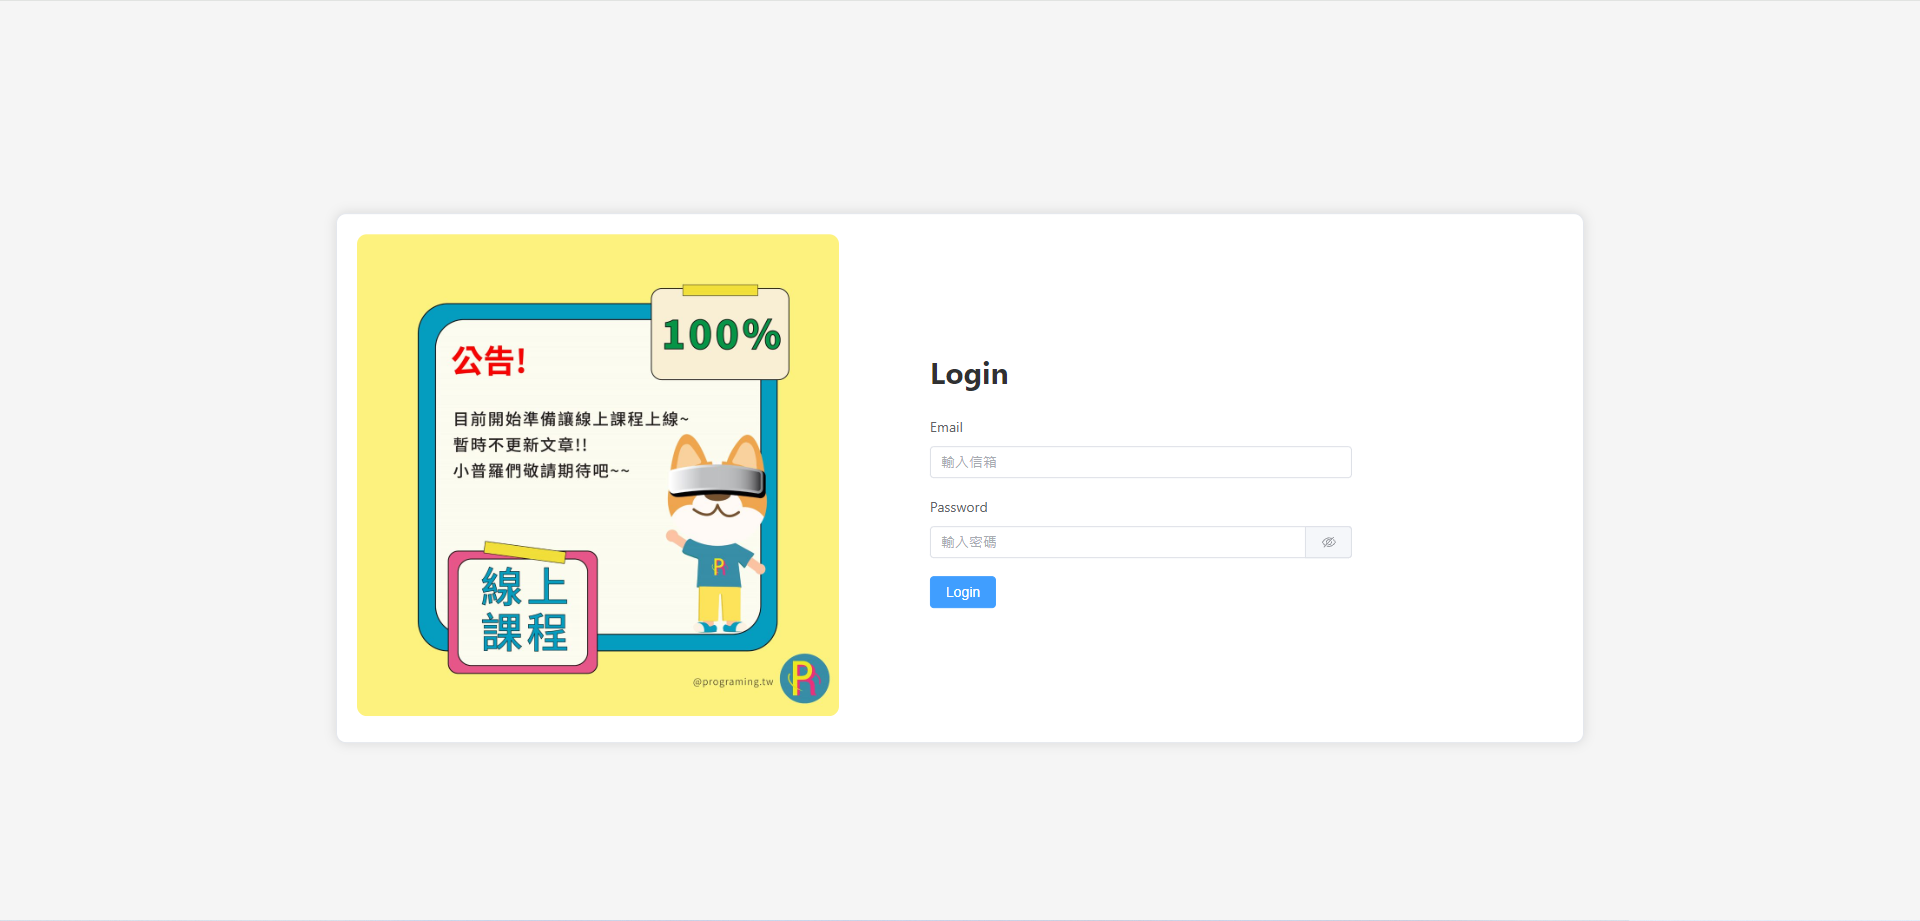
\includegraphics[width=0.60\textwidth]{./img/login.png}
  }
  \caption{登入頁面 (點擊可看大圖)}
\end{figure}

\subsection{進入課程}
登入後,點擊想要進入的課程卡片。

\begin{figure}[H]
  \centering
  \href{https://raw.githubusercontent.com/programingtw/proglearn-plan/main/2023全國大專校院智慧創新暨跨域整合創作競賽/img/course.png}{
    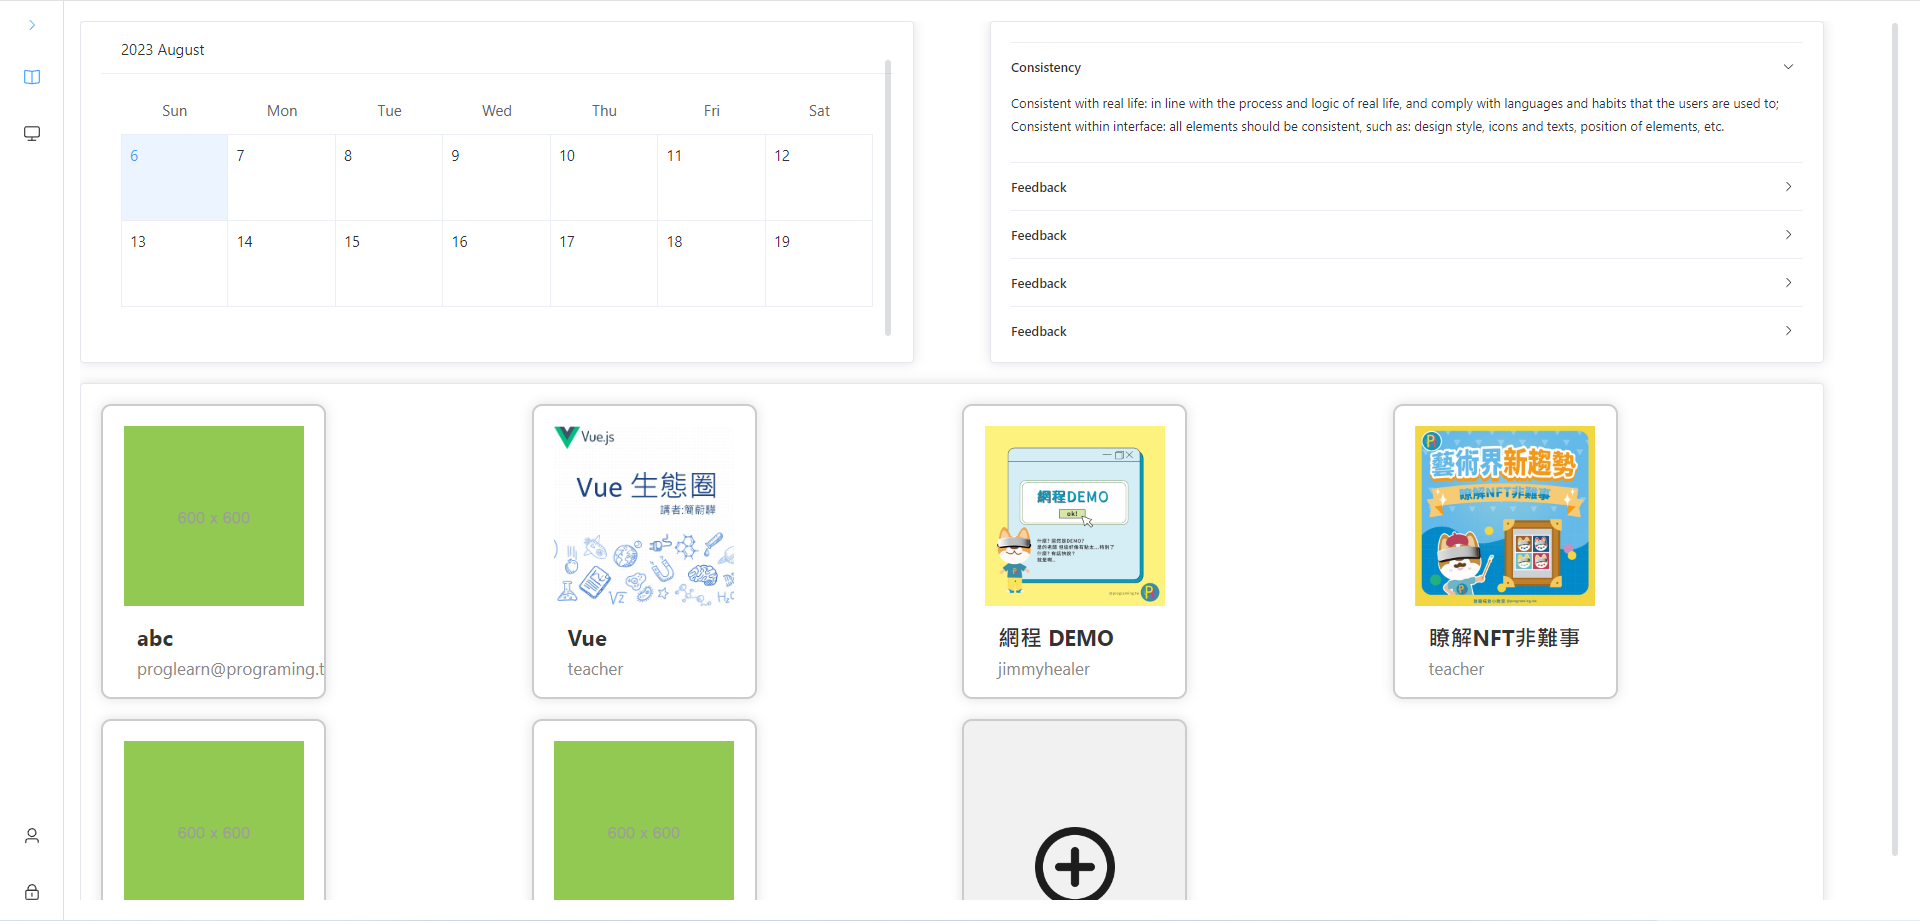
\includegraphics[width=0.60\textwidth]{./img/course.png}
  }
  \caption{課程列表頁面 (點擊可看大圖)}
\end{figure}

\subsection{老師操作}

\subsubsection{新增課程}
在主畫面點擊新增課程卡片,填入課程相關資訊,點擊儲存按鈕,新課程被創建。

\begin{figure}[H]
  \centering
  \href{https://raw.githubusercontent.com/programingtw/proglearn-plan/main/2023全國大專校院智慧創新暨跨域整合創作競賽/img/addCourse.png}{
    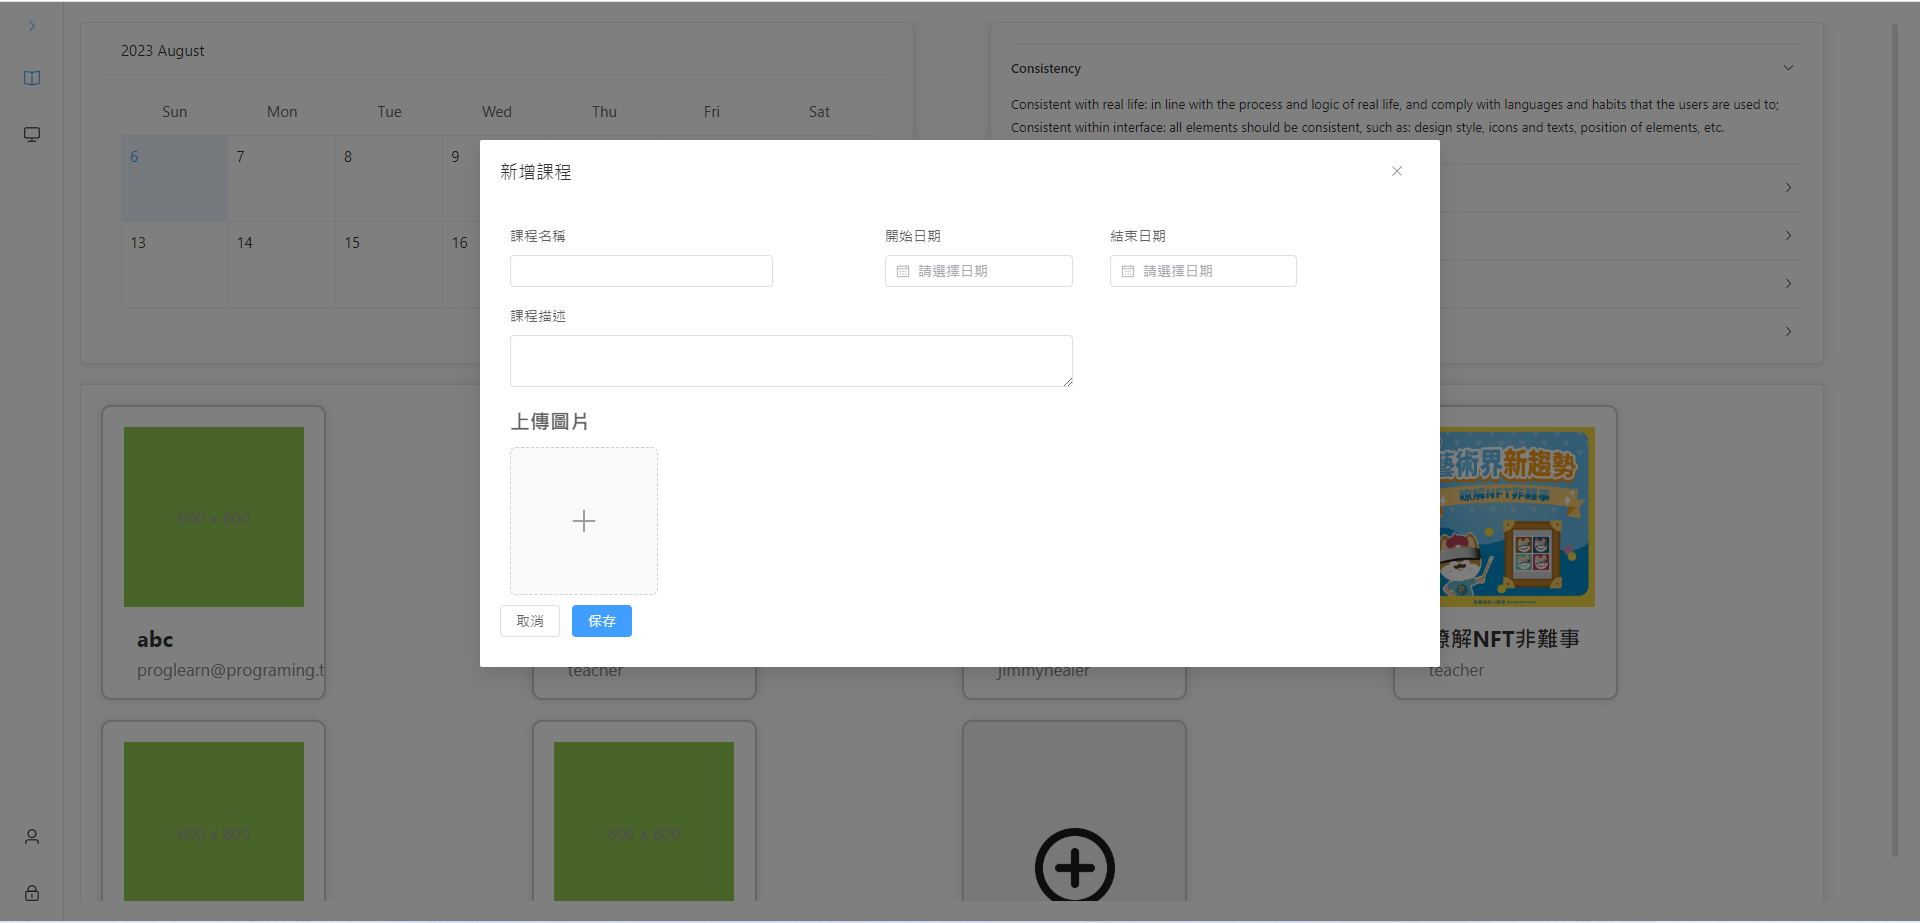
\includegraphics[width=0.60\textwidth]{./img/addCourse.png}
  }
  \caption{新增課程頁面 (點擊可看大圖)}
\end{figure}

\subsubsection{新增章節及教材}
在課程頁面點擊新增章節按鈕,填入章節名稱並上傳講義,點擊儲存按鈕。
根據要上傳的教材類型點擊章節下的按鈕,選擇檔案並上傳。

\begin{figure}[H]
  \centering
  \href{https://raw.githubusercontent.com/programingtw/proglearn-plan/main/2023全國大專校院智慧創新暨跨域整合創作競賽/img/chapter.png}{
    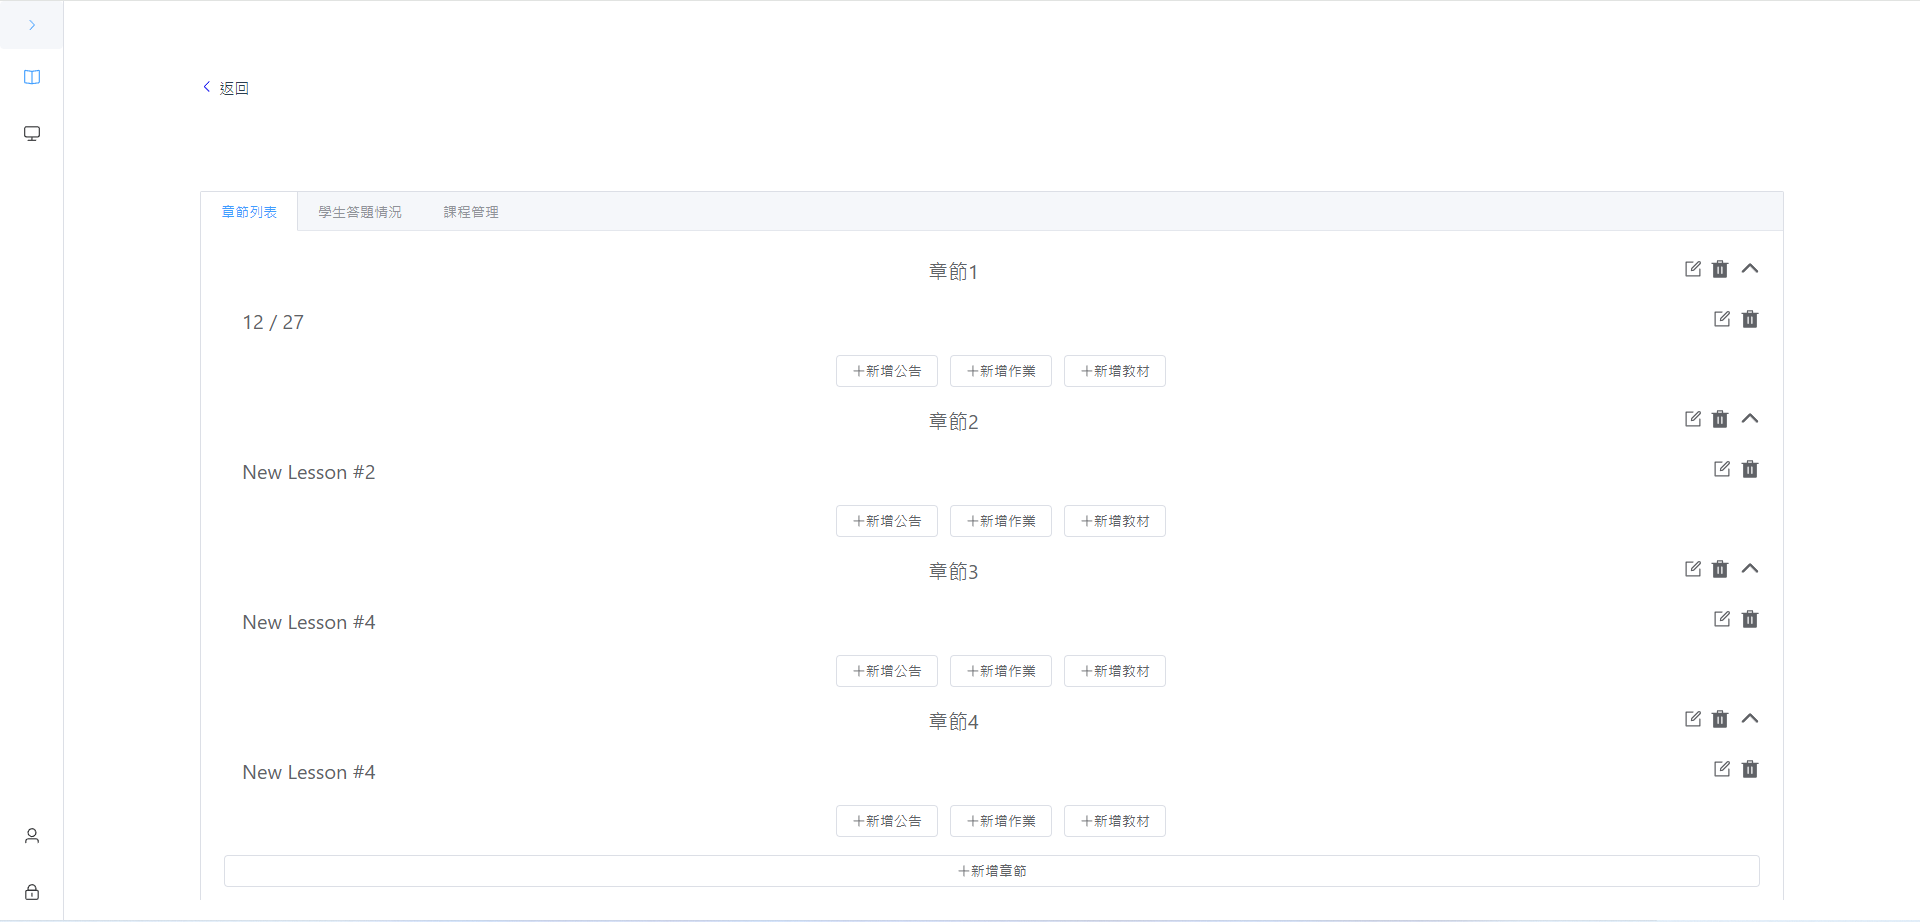
\includegraphics[width=0.60\textwidth]{./img/chapter.png}
  }
  \caption{章節列表頁面 (點擊可看大圖)}
\end{figure}

\subsubsection{編輯講義}
在編輯頁面,以積木方式分塊內容,方塊區選擇添加方塊類型,編輯區編輯內容。
利用時間軸編輯控制顯示區段,編輯完成後點擊儲存按鈕。

\begin{figure}[H]
  \centering
  \href{https://raw.githubusercontent.com/programingtw/proglearn-plan/main/2023全國大專校院智慧創新暨跨域整合創作競賽/img/teacher2.png}{
    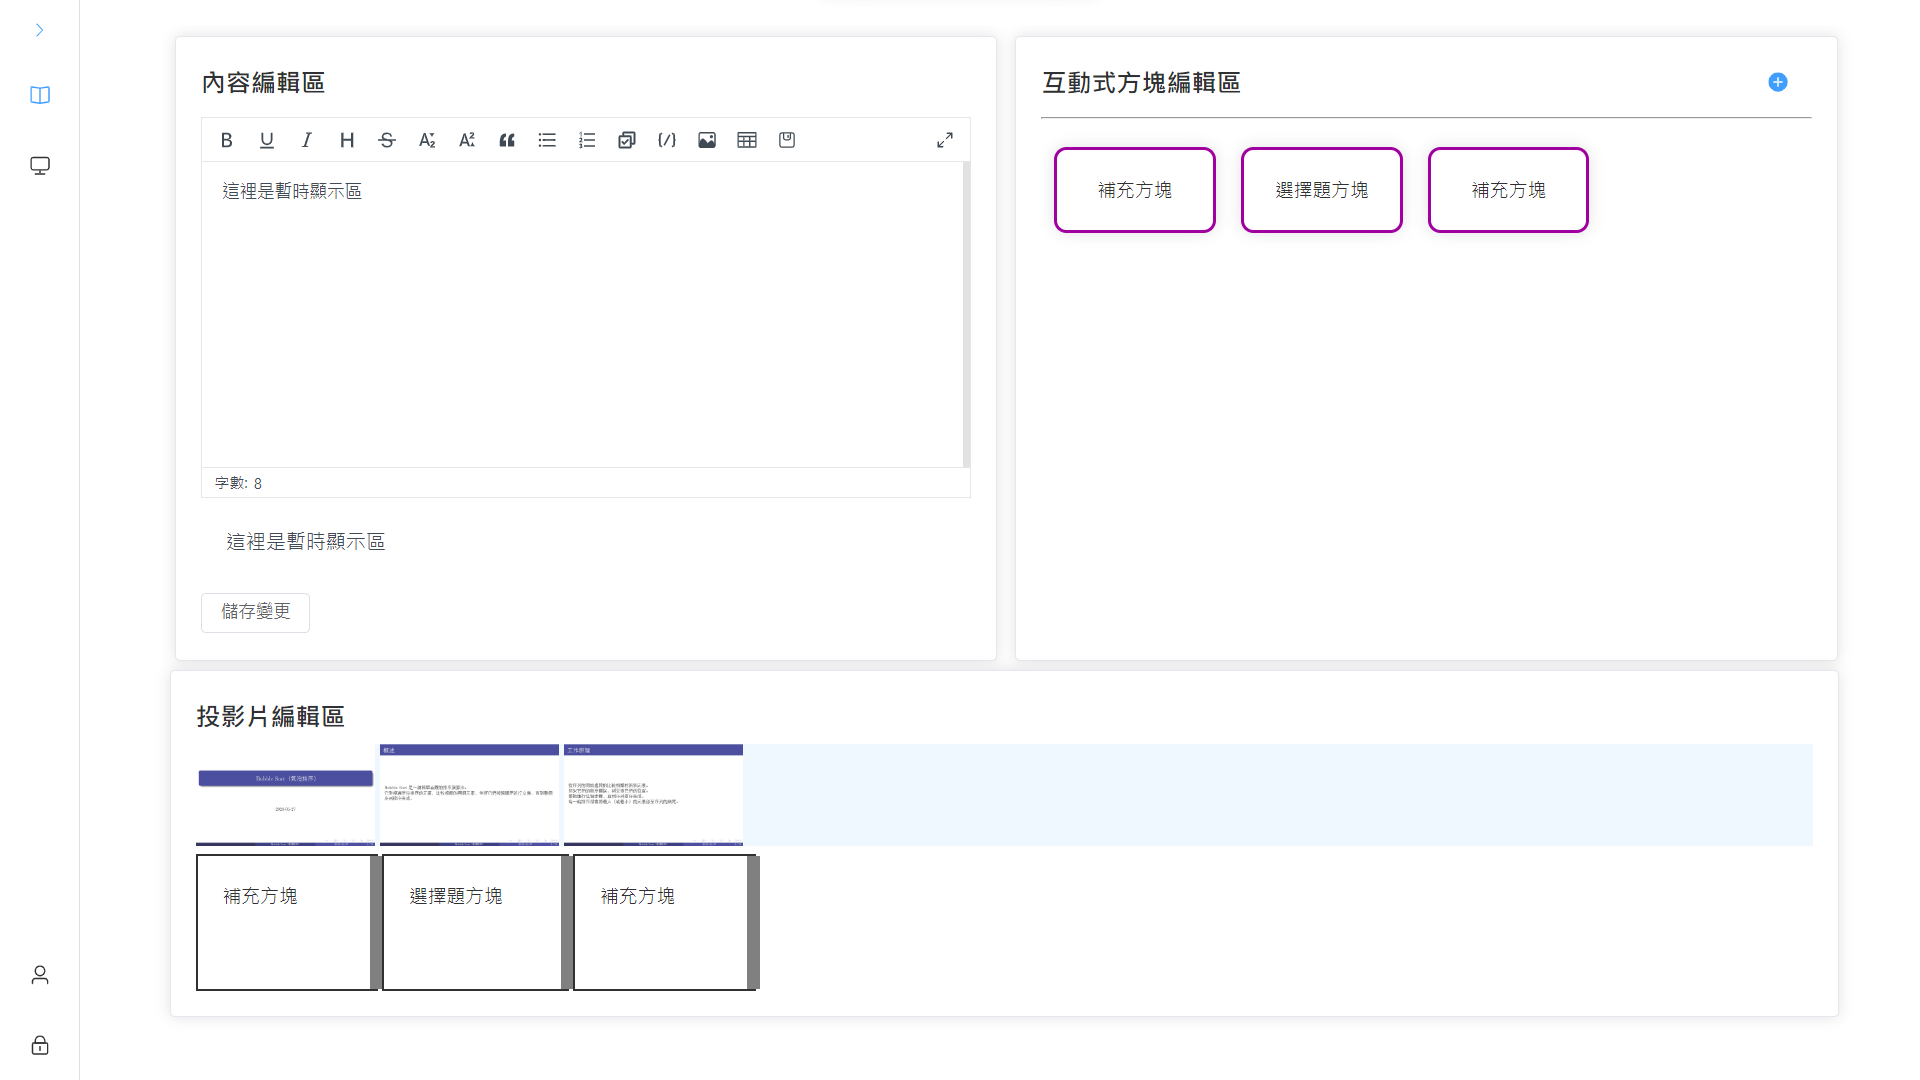
\includegraphics[width=0.60\textwidth]{./img/teacher2.png}
  }
  \caption{教師講義編輯頁面 (點擊可看大圖)}
\end{figure}

\subsubsection{上課及查看學生狀況}

\begin{itemize}
  \item 點擊「開始授課」按鈕,系統開始記錄。
  \item 在課堂練習開放後查看學生答題狀況。
  \item 課程結束點擊「結束授課」按鈕。
\end{itemize}

\begin{figure}[H]
  \centering
  \href{https://raw.githubusercontent.com/programingtw/proglearn-plan/main/2023全國大專校院智慧創新暨跨域整合創作競賽/img/teacher.png}{
    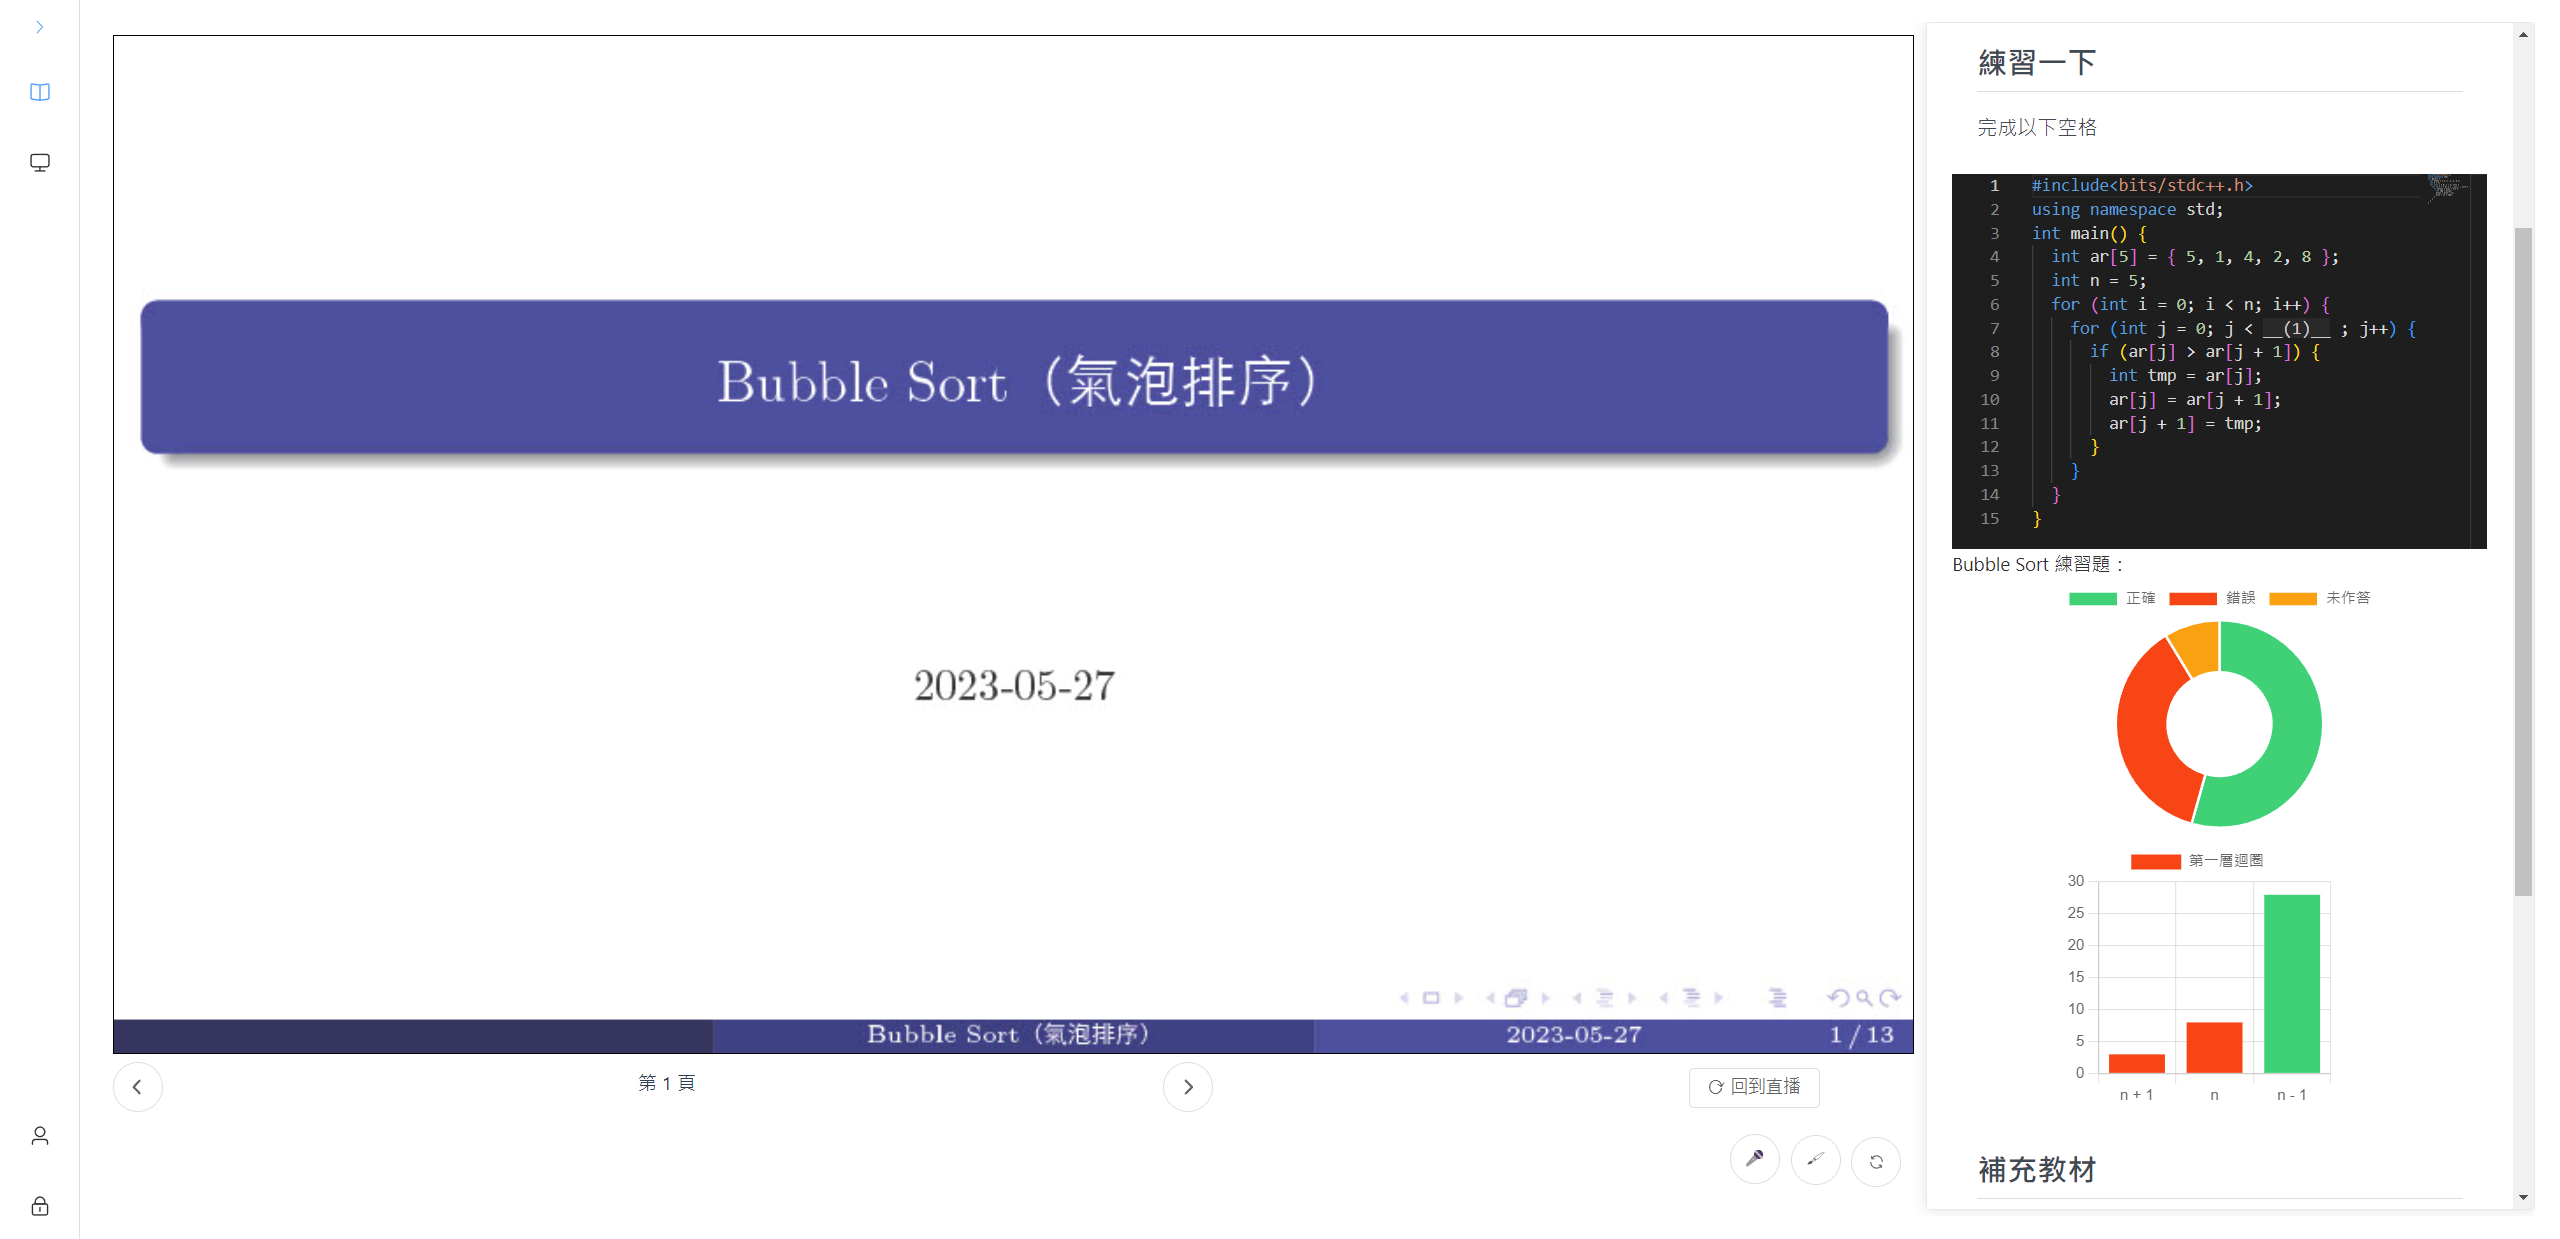
\includegraphics[width=0.60\textwidth]{./img/teacher.png}
  }
  \caption{教師上課頁面 (點擊可看大圖)}
\end{figure}

\subsection{學生操作}
\subsubsection{上課及課堂互動}
進入課程頁面上課,引導模式查看老師當前進度。
老師展示練習題時,選擇答案並提交。

\begin{figure}[H]
  \centering
  \href{https://raw.githubusercontent.com/programingtw/proglearn-plan/main/2023全國大專校院智慧創新暨跨域整合創作競賽/img/student2.png}{
    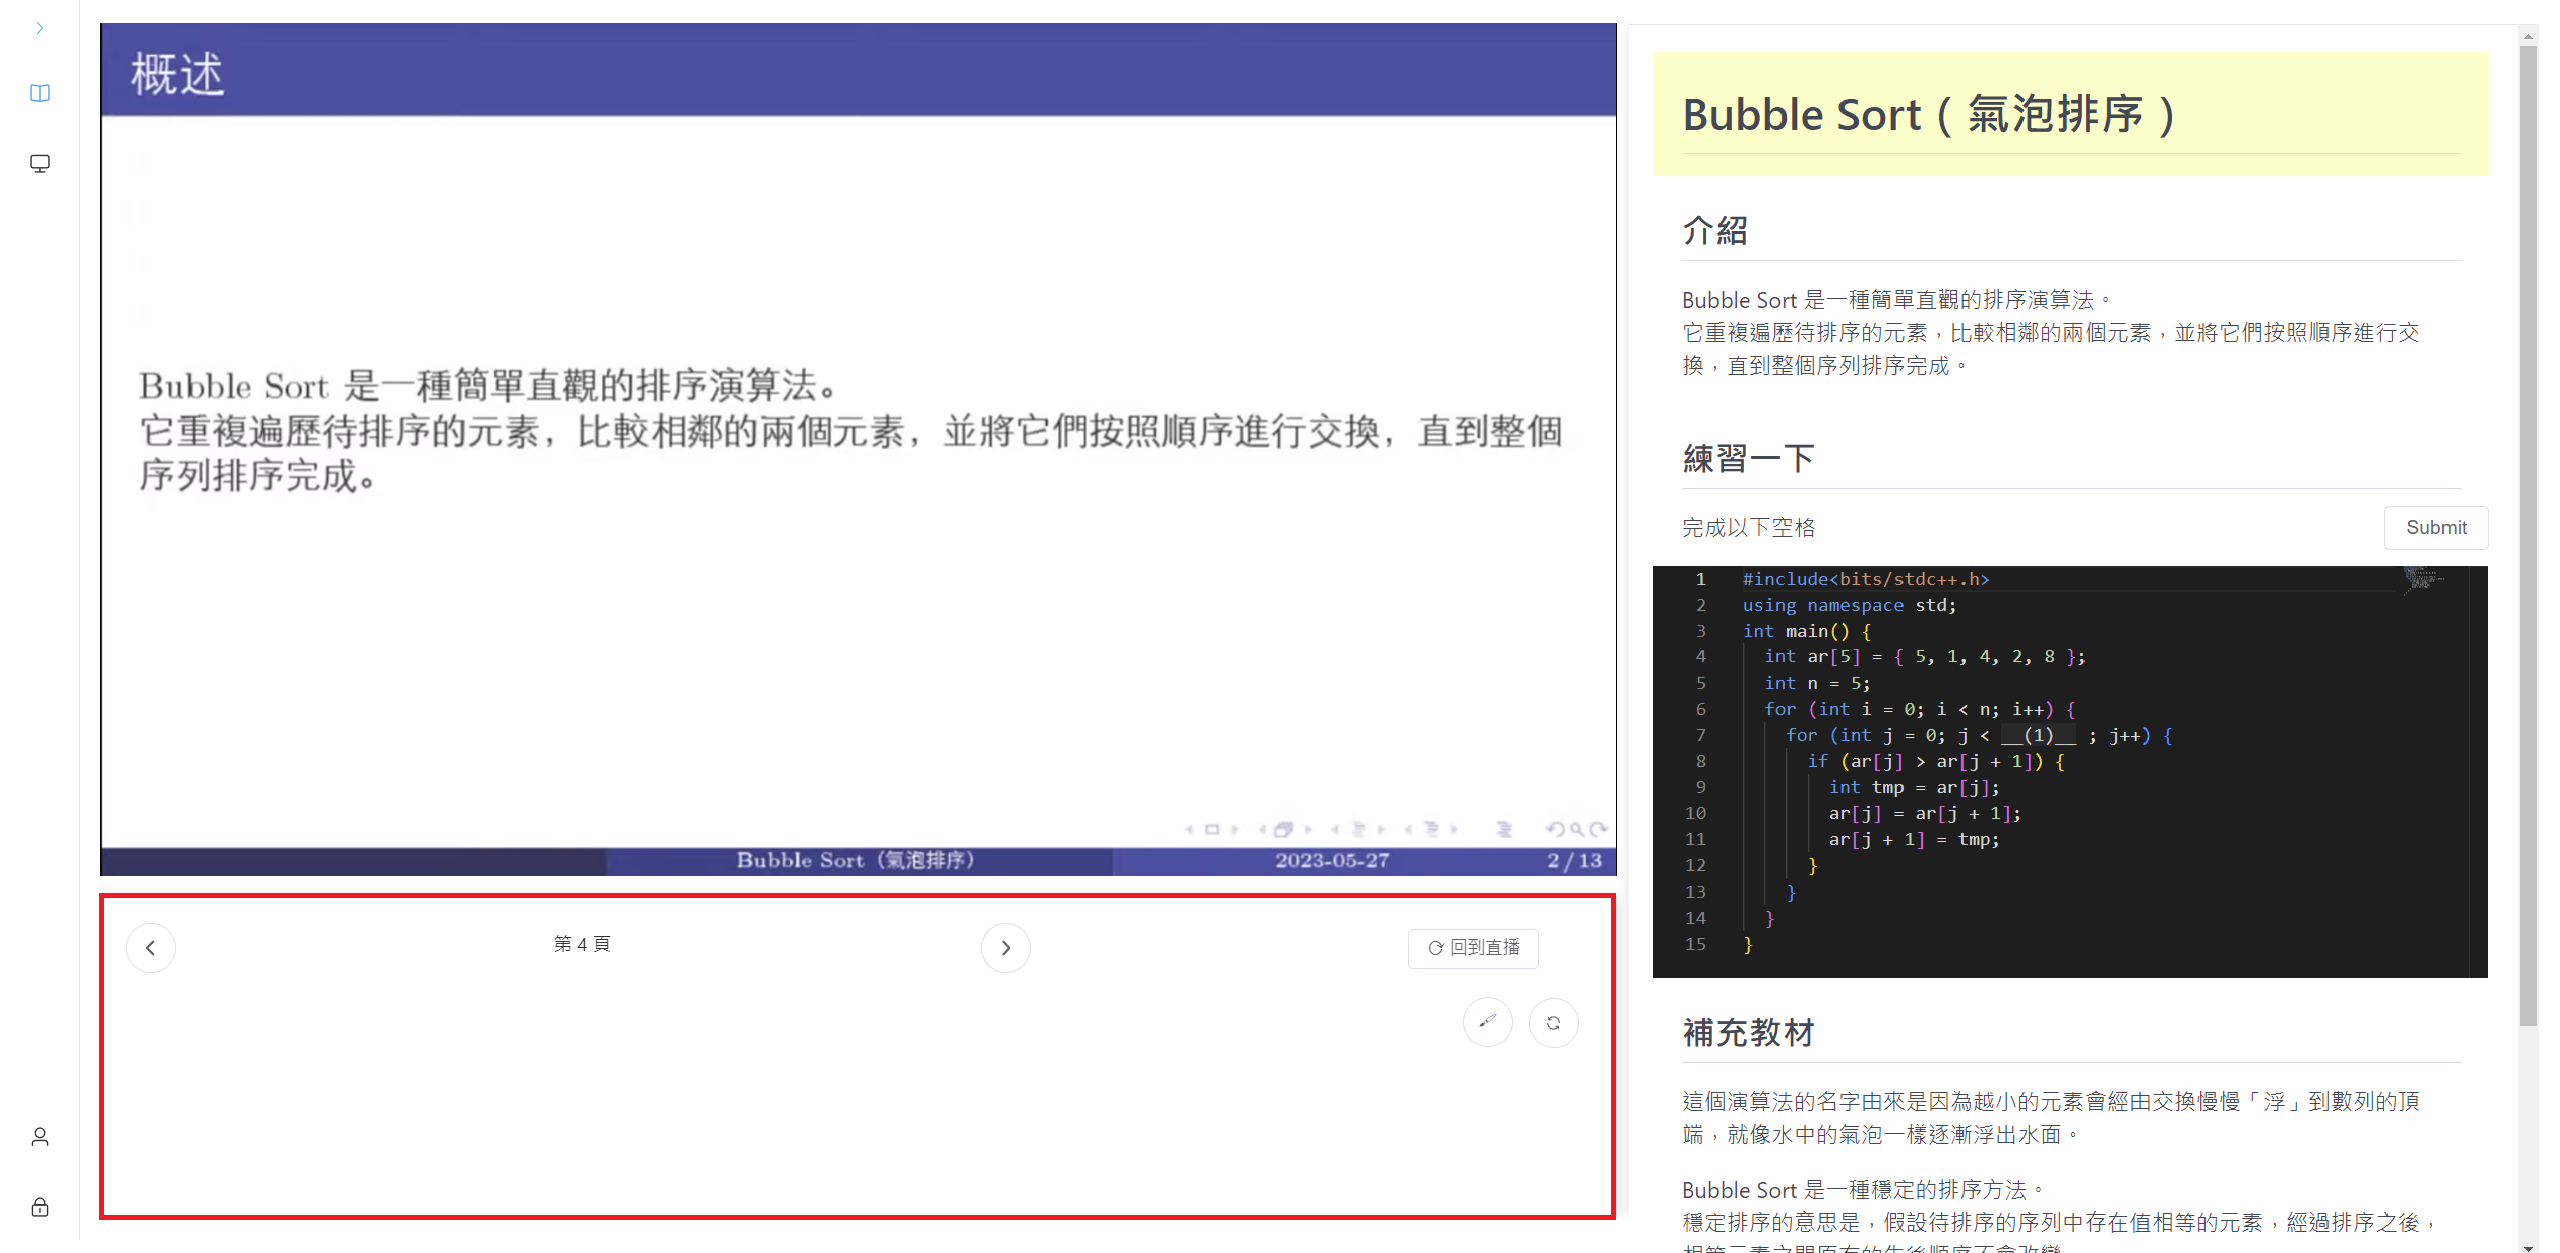
\includegraphics[width=0.60\textwidth]{./img/student2.png}
  }
  \caption{學生上課頁面 (點擊可看大圖)}
\end{figure}

\subsubsection{課後複習}
回到教學頁面,播放錄影,回答練習題。

\begin{figure}[H]
  \centering
  \href{https://raw.githubusercontent.com/programingtw/proglearn-plan/main/2023全國大專校院智慧創新暨跨域整合創作競賽/img/student3.png}{
    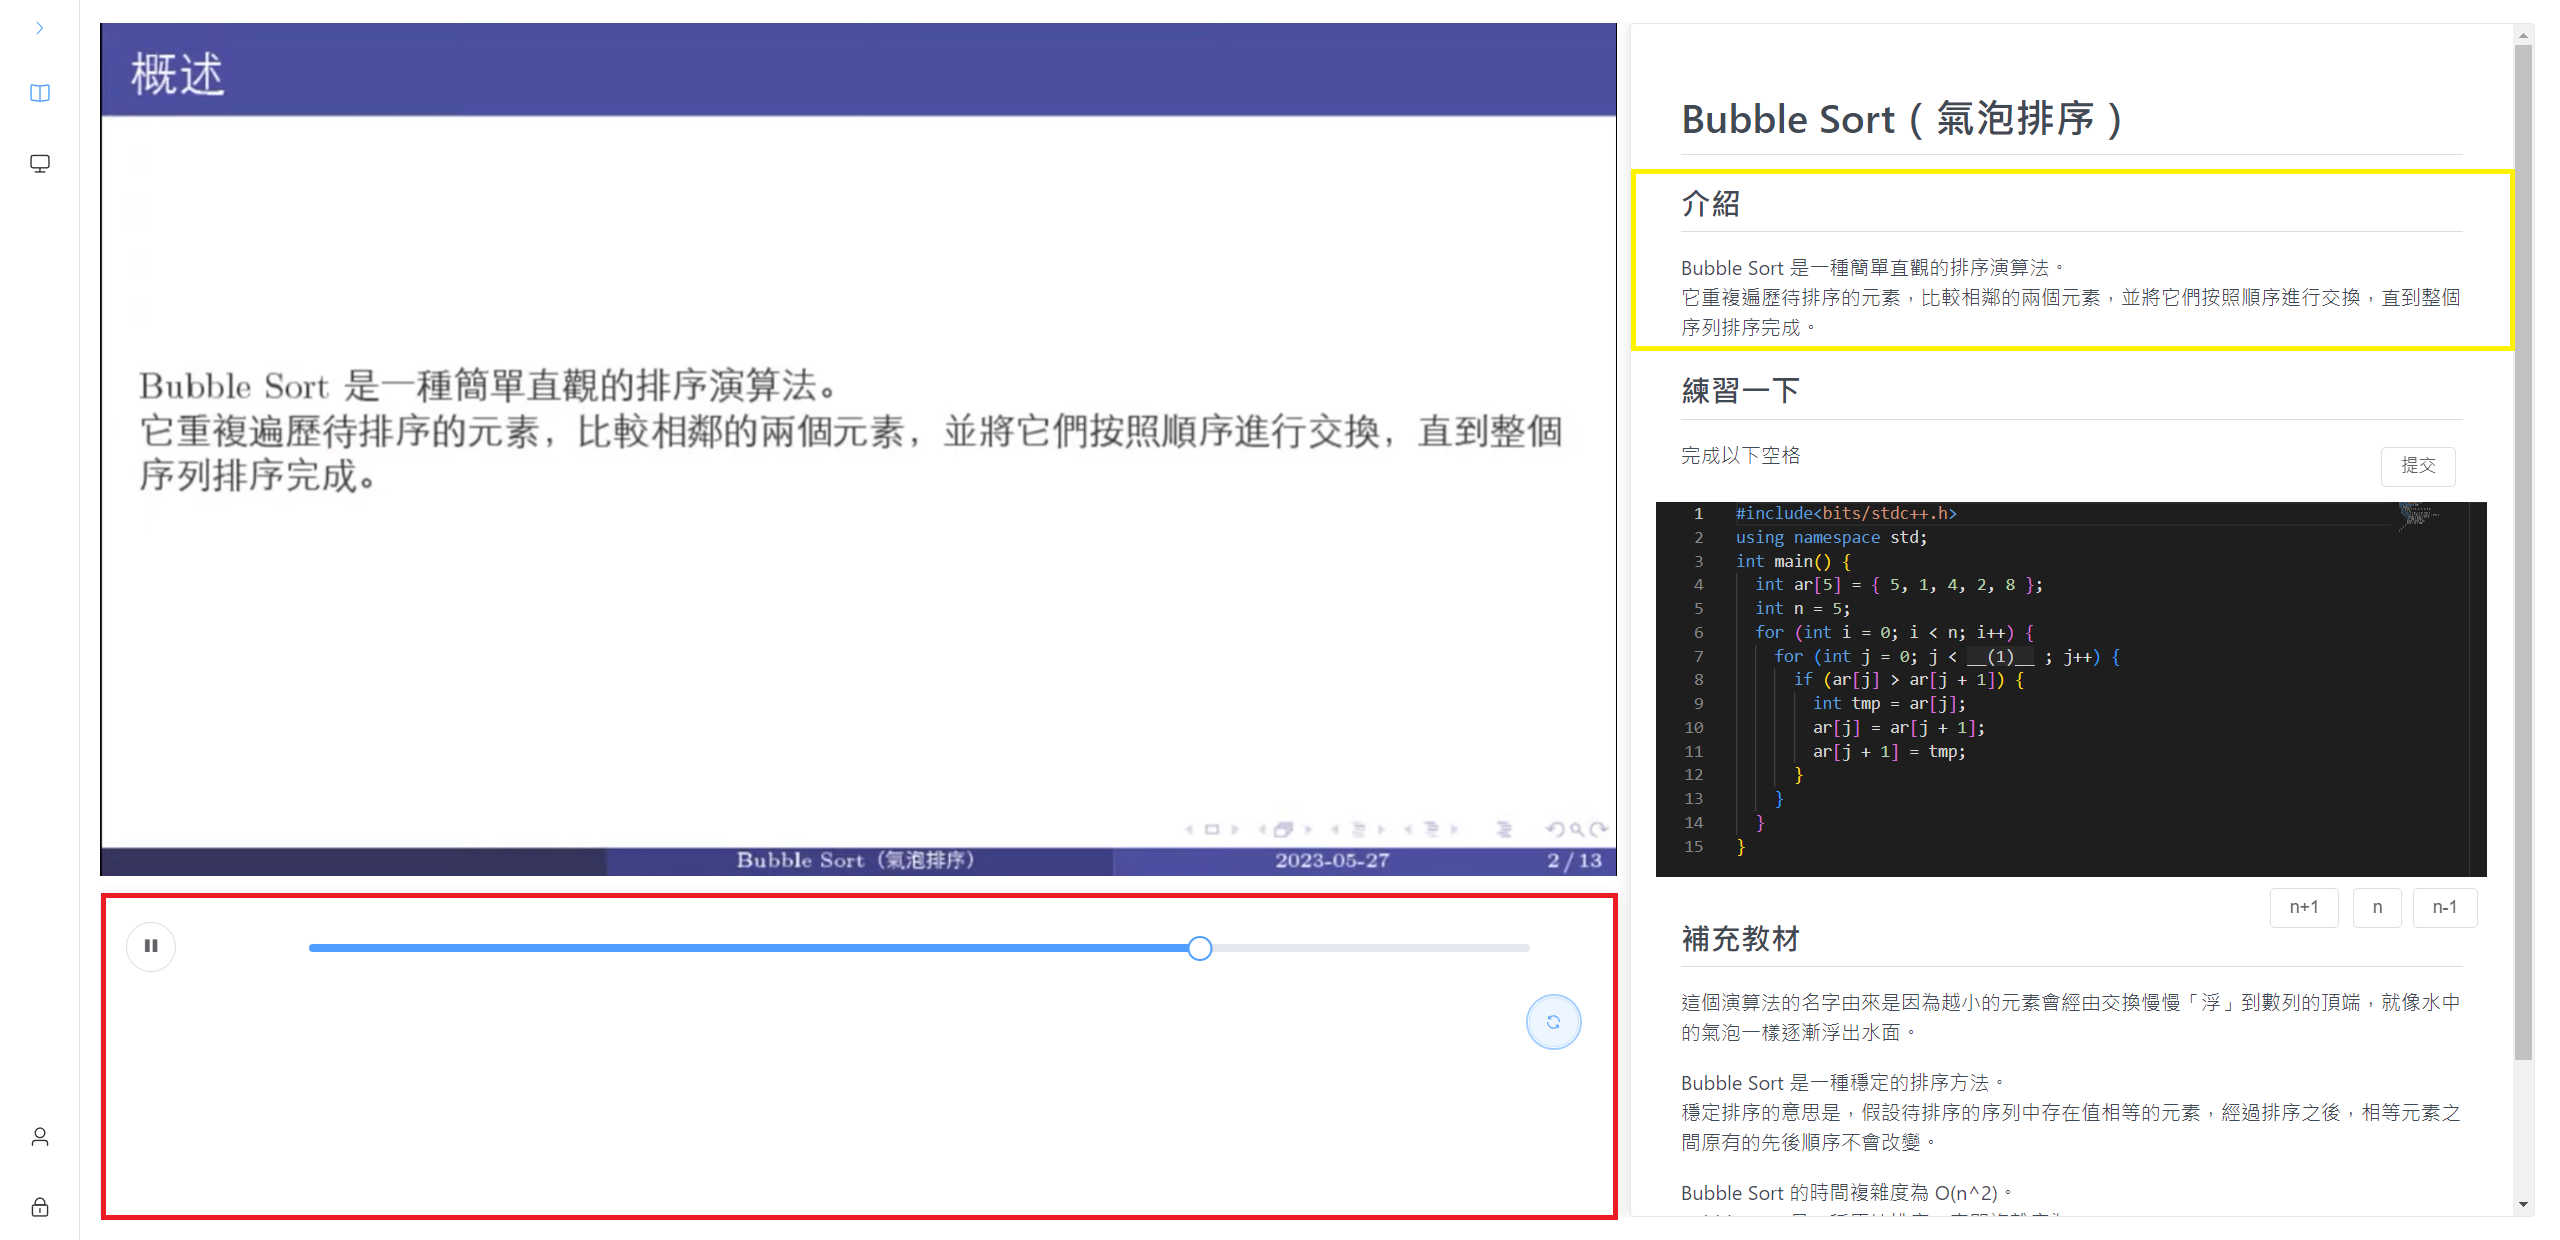
\includegraphics[width=0.60\textwidth]{./img/student3.png}
  }
  \caption{學生課後複習頁面 (點擊可看大圖)}
\end{figure}
  
\end{document}